\subsection{Multi-Agent Proximal Policy Optimization}
\label{subsec:41}

Since the naive application of standard reinforcement learning algorithms performs poorly in multi-agent settings, our goal is to derive an algorithm that can operate under the following constraints:
\begin{itemize}
\item{The learned policies can only use local information (i.e. own observations) at execution time.}
\item{There is no particular communication method between the agents, since it can restrict the scalability of the solution.}
\item{We do not assume a differential model of the environment dynamics.}
\end{itemize}
Fulfilling the above desiderata would provide a general-purpose multi-agent learning algorithm that could be applied not just to cooperative games with explicit communication channels, but also to competitive games and games involving only physical interactions between agents.

We accomplish our goal by adopting the framework of centralized training with decentralized execution in which agent policies are composed of two separate networks with different parameters: a policy network (actor) that generates an action distribution and a critic network (critic) that predicts discounted future returns. The critic uses extra information to ease training process whilst actors take actions based solely on their own local observations. This is still a valid approach as long as the information used during the training of the agents are not used at test/execution time.

% For figures use
%
\begin{figure}[h!]
%\sidecaption
% Use the relevant command for your figure-insertion program
% to insert the figure file.
% For example, with the graphicx style use
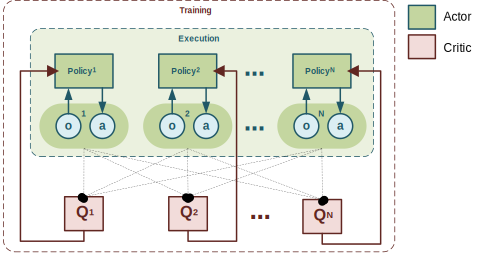
\includegraphics[scale=.65]{images/MAPPO}
%
% If no graphics program available, insert a blank space i.e. use
%\picplace{5cm}{2cm} % Give the correct figure height and width in cm
%
\caption{Overview of our multi-agent decentralized actor, centralized critic approach. The centralized action-value function (critic) for each agent takes as input the actions and observations of all agents and predicts the discounted future returns (Q-values) for the agent while the actor produces an action distribution based solely on the agent's observations and actions.}
\label{fig:MAPPO}       % Give a unique label
\end{figure}

As illustrated in Fig. \ref{fig:MAPPO}, our centralized action-value function (critic) for each agent takes as input the actions and observations of all agents and predicts the discounted future returns for the agent. Additional information can also be included in the inputs. Since each action-value function is learned separately, each agent can have arbitrary rewards including conflicting rewards in competitive scenarios.

Furthermore, we extend the idea of \cite{schulman2017proximal} by adopting the proximal policy optimization algorithm (PPO) as the main policy optimization algorithm instead of deep deterministic policy gradient (DDPG) as presented in the paper. PPO is a family of policy optimization methods that use multiple epochs of stochastic gradient ascent to perform each policy update. It performs comparably to or better than DDPG while being much simpler to implement and tune.

\subsection{Cooperation and Competition}
\label{subsec:42}
As we seek the emergence of coordination strategies between the components of the micro-grid, the agents controlling the mico-grid components are trained using \textit{self-play} in an \textit{autocuricula} configuration. This acts as a natural curriculum as these agents are always in a mixed cooperative and competitive setting. For example, the energy loads (i.e. production machines) of the micro-grid are always in competitive settings. If there is not enough electrical energy available in the grids, then some production machines have to turn themselves off so that the production can be carried on by the other machines. In the same direction, cooperation can take place if, for example, the energy storage components need to be switched to the discharging state in order to increase the electrical energy available on the energy bus and thus enable the production machines to perform additional production tasks.

Adopting such a configuration also offers many advantages. If a new successful strategy is adopted by an agent, it implicitly changes the task distribution for the competing agents which are then forced to develop a better strategy. These evolutionary arms races create an implicit autocurriculum in which competing agents constantly create new tasks for each other and thus discover new powerful and robust strategies and counter-strategies. In addition, the multi-agent autocurriculum is open-ended. That means that the training will only stabilizes once equilibrium between the different agents is founded which can only be reached if a suitable coordination strategy between the agents has emerged. Due to the exploration factors, many coordination strategies can also emerge at different stages of the training.

In order to create a competitive setting, competing agents are rewarded with competitive rewards. If an agent wins the game, it receives a positive reward and all other competing agents are penalized by an opposite negative reward. If nobody wins the game, then all competing agent are penalized. In a cooperative setting, agents are given a team based reward; meaning that all members of the team receive a positive reward, if a team member wins the game. To confine agent behavior to a reasonable space, we also introduced an environmental-based penalization.

The success of agents in the autocuricula setting requires the agents to occasionally solve the task (win the game) by random actions. The probability of this happening in most games is minuscule as they require as a prerequisite some fundamental skills like the ability to properly control the operational state machine of the grid component. For example the agent must first quickly learn how to bring a production machine in the $execute$-state in order to start a production task or how to turn on/off the storage component without suspending/halting the production. To overcome this problem, we use simple dense rewards at each step so that the agents can first learn basic motor skills that increase the likelihood that random actions of the agent will result in a relatively small positive reward. We refer to this reward as the \textit{exploration reward}. The exploration reward is then gradually annealed to zero, in favor of the \textit{competition/cooperation reward}, to allow the agents to learn coordination strategies for the remaining training time. This is achieved using a linear annealing factor $\alpha$. We also introduce an \textit{environmental reward} which aims to penalize action sequences leading to dangerous outcomes (for example system configurations violating the constraints formulated in Eq. \ref{eq:constraint_energy_balance} and Eq. \ref{eq:constraint_load_profile}) and a \textit{productivity reward} which encourage production machines to execute production tasks more frequently. 

So, at time-step $t$, if the exploration reward is $r_{explo}$, the competition reward is $r_{comp}$, the environmental reward $r_{env}$, the the productivity reward $r_{prod}$ and T is the termination time-step, then the total agent reward is:
\begin{equation}
\label{eq:total_reward}	
	r_t = \alpha \cdot r_{explo} + (1 - \alpha) \cdot (r_{comp} + r_{env} + r_{prod})
\end{equation} 

With this formulation, the agents are trained initially on the dense reward for only about 10-20\% of the training epochs in order to gain some basic skills first. 
